
\section{Result: DMPcreator}
The result of our implementation efforts is the user friendly webinterface \texttt{DMPcreator}. The tool is structured into five slides. Every slide...\\
The first slide, the \textit{General Information Slide}~\ref{GeneralInformationSlide}, provides fields letting the user enter general information about his project, for example the project name, the person in charge of the project and contact data. Furthermore, the user can upload his .TSV file created by \texttt{Q-Wizard}. One important topic that needs to be covered when creating a data management plan is \textit{Roles \& Responsibilities}~\ref{RolesResponsibilitiesSlide}. This second slide allows the user to assign roles to persons. The chosen values are added two a responsibilities list. Having specified who is responsible for which data, the user still has to decide, how the data is stored. Here comes the third slide \textit{ContentManagement} in handy.
\begin{figure}[]
	\centering
    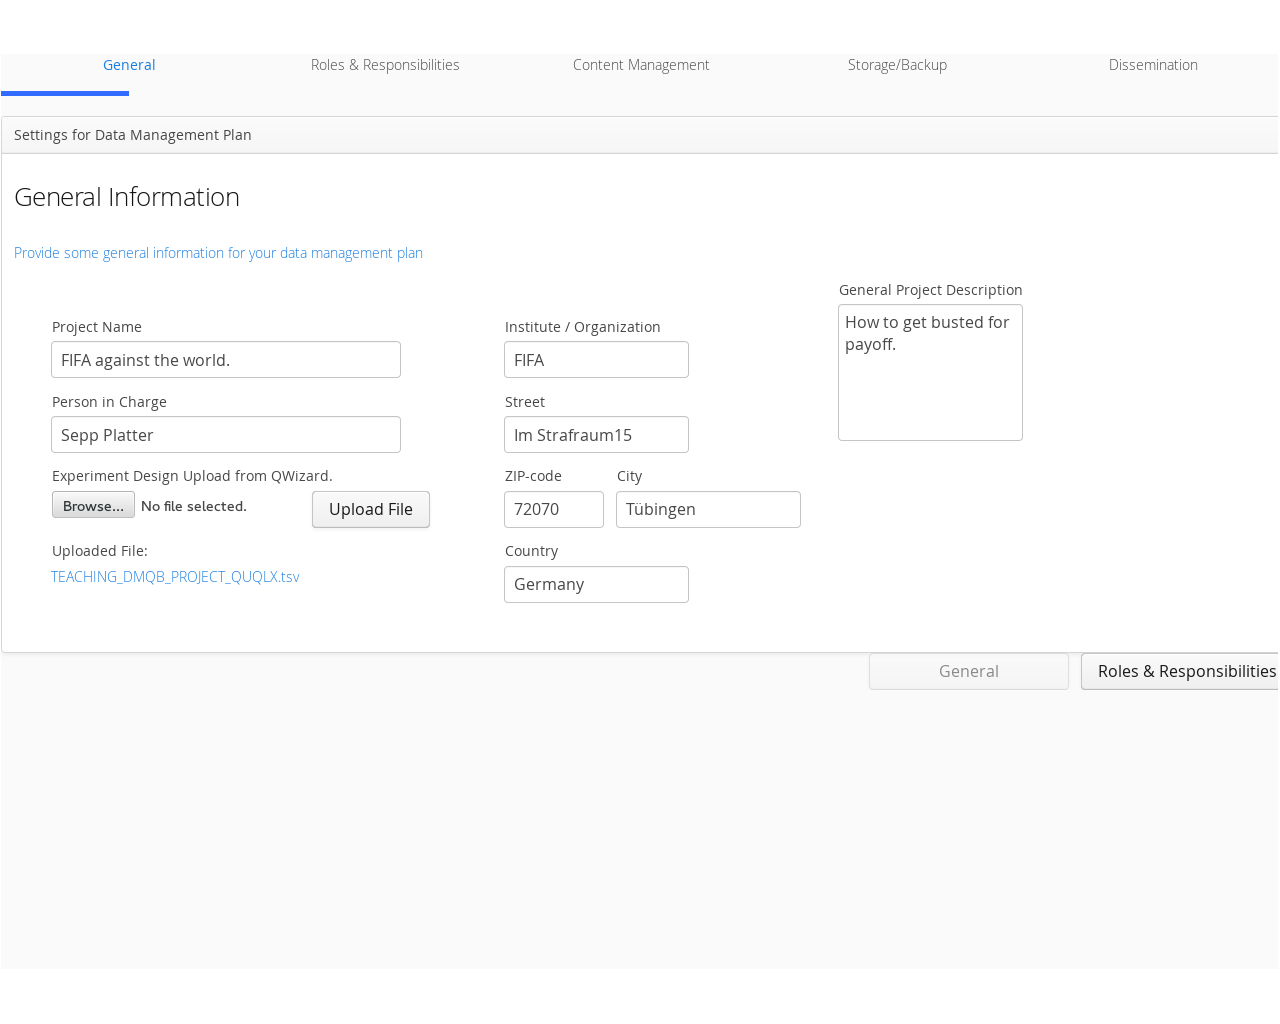
\includegraphics[width=0.7\textwidth]{pictures/GeneralInformation.png}
    \caption{General Information Slide of \texttt{DMPcreator}. The progress bar is placed on the top. Fields that are fillable by the user can be seen below. Note, a special upload field for the .TSV file from \texttt{Q-Wizard} is visible on the left bottom.}
    \label{GeneralInformationSlide}
\end{figure}

\begin{figure}[]
	\centering
	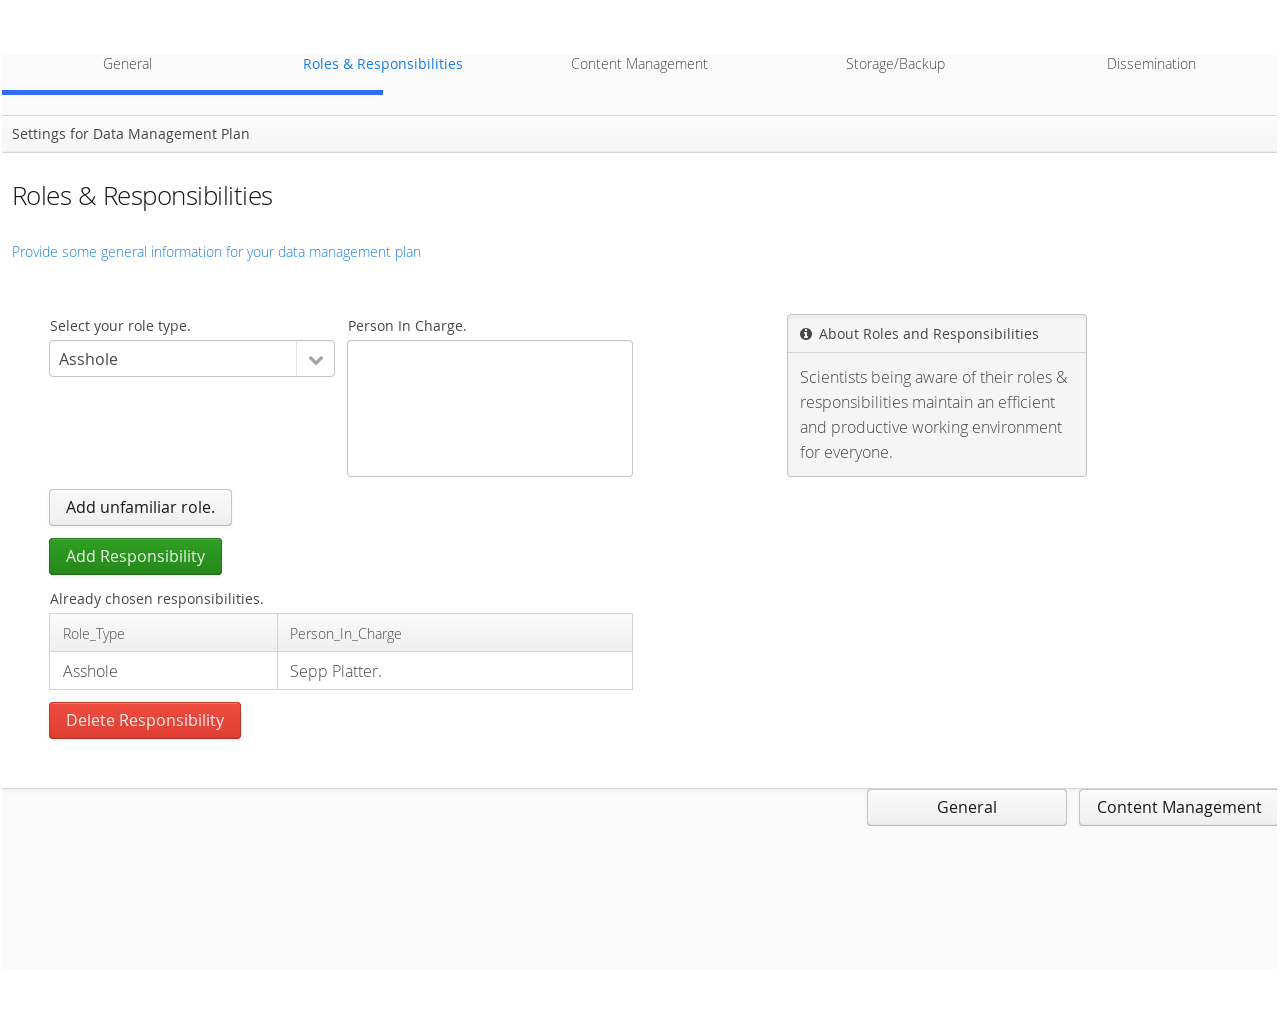
\includegraphics[width=0.7\textwidth]{pictures/RolesResponsibilities.png}
	\caption{Roles \& Responsibilities Slide of \texttt{DMPcreator}. The progress bar is placed on the top. Fields that are fillable by the user can be seen below.}
	\label{RolesResponsibilitiesSlide}
\end{figure}

\begin{figure}[]
	\centering
	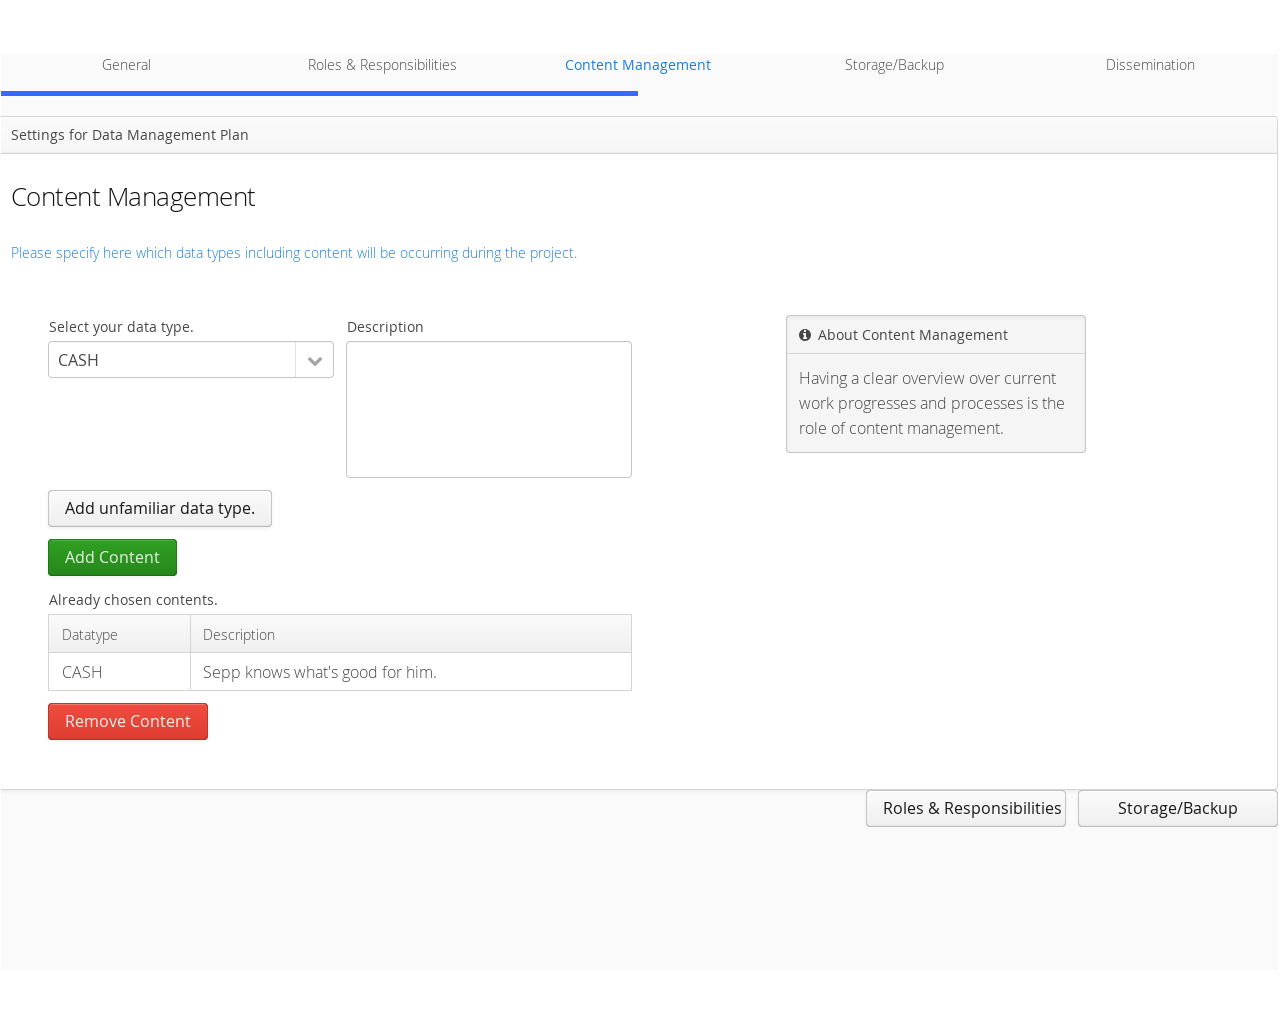
\includegraphics[width=0.7\textwidth]{pictures/ContentManagement.png}
	\caption{General Information Slide of \texttt{DMPcreator}. The progress bar is placed on the top. Fields that are fillable by the user can be seen below.}
	\label{ContentManagementSlide}
\end{figure}

\begin{figure}[]
	\centering
	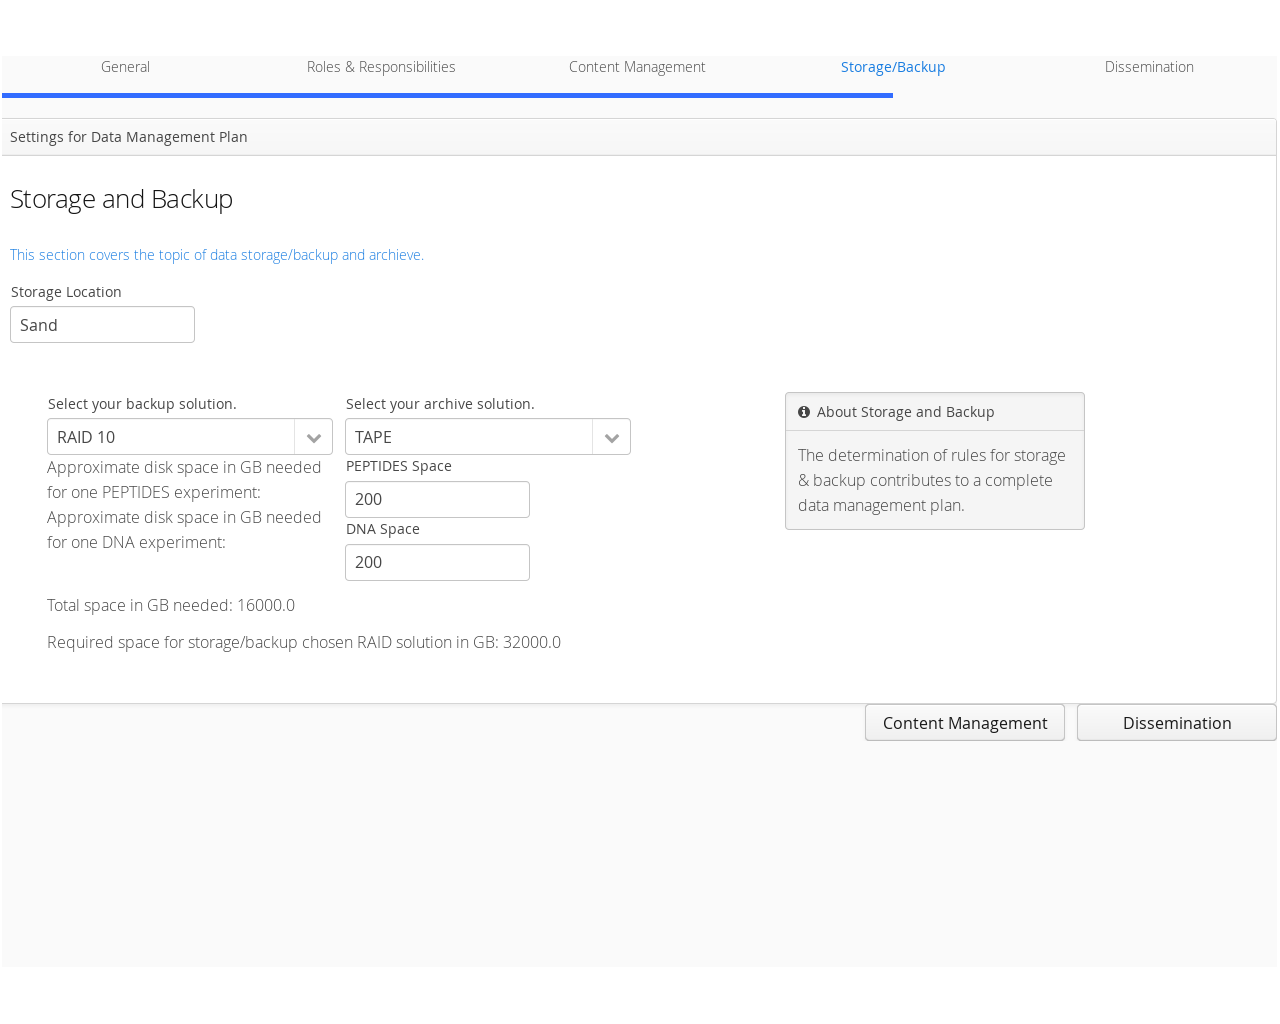
\includegraphics[width=0.7\textwidth]{pictures/StorageBackup.png}
	\caption{General Information Slide of \texttt{DMPcreator}. The progress bar is placed on the top. Fields that are fillable by the user can be seen below.}
		\label{StorageBackupSlide}
\end{figure}

\begin{figure}[]
	\centering
	\label{Dissemination}
	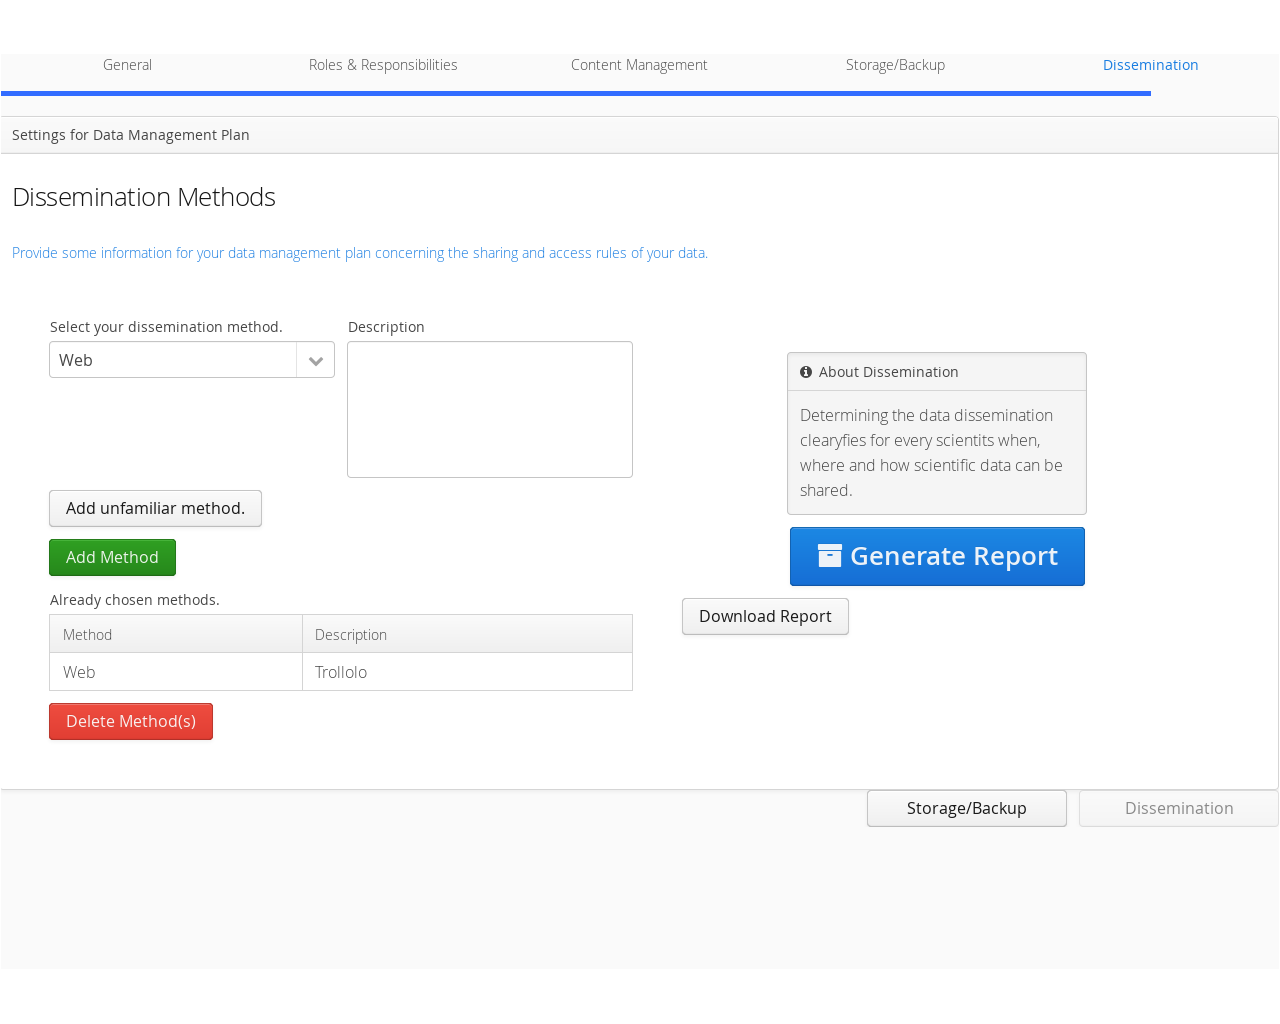
\includegraphics[width=0.7\textwidth]{pictures/Dissemination.png}
	\caption{General Information Slide of \texttt{DMPcreator}. The progress bar is placed on the top. Fields that are fillable by the user can be seen below.}
\end{figure}